%conjunct analysis
After obtaining neural and behavioral loss aversion, by conjunction analysis, two figures below are generated to show the relationships between neural and behavioral loss aversion. Each plot contains three subplots for each run. Since two types of regression methods, original least square and robust regression, are performed, we obtain two regression line. The black line is for OLS, while the blue line is for robust regression. In the plots, the outliers are labeled as red dots. 

\begin{figure}[h!]
\centering
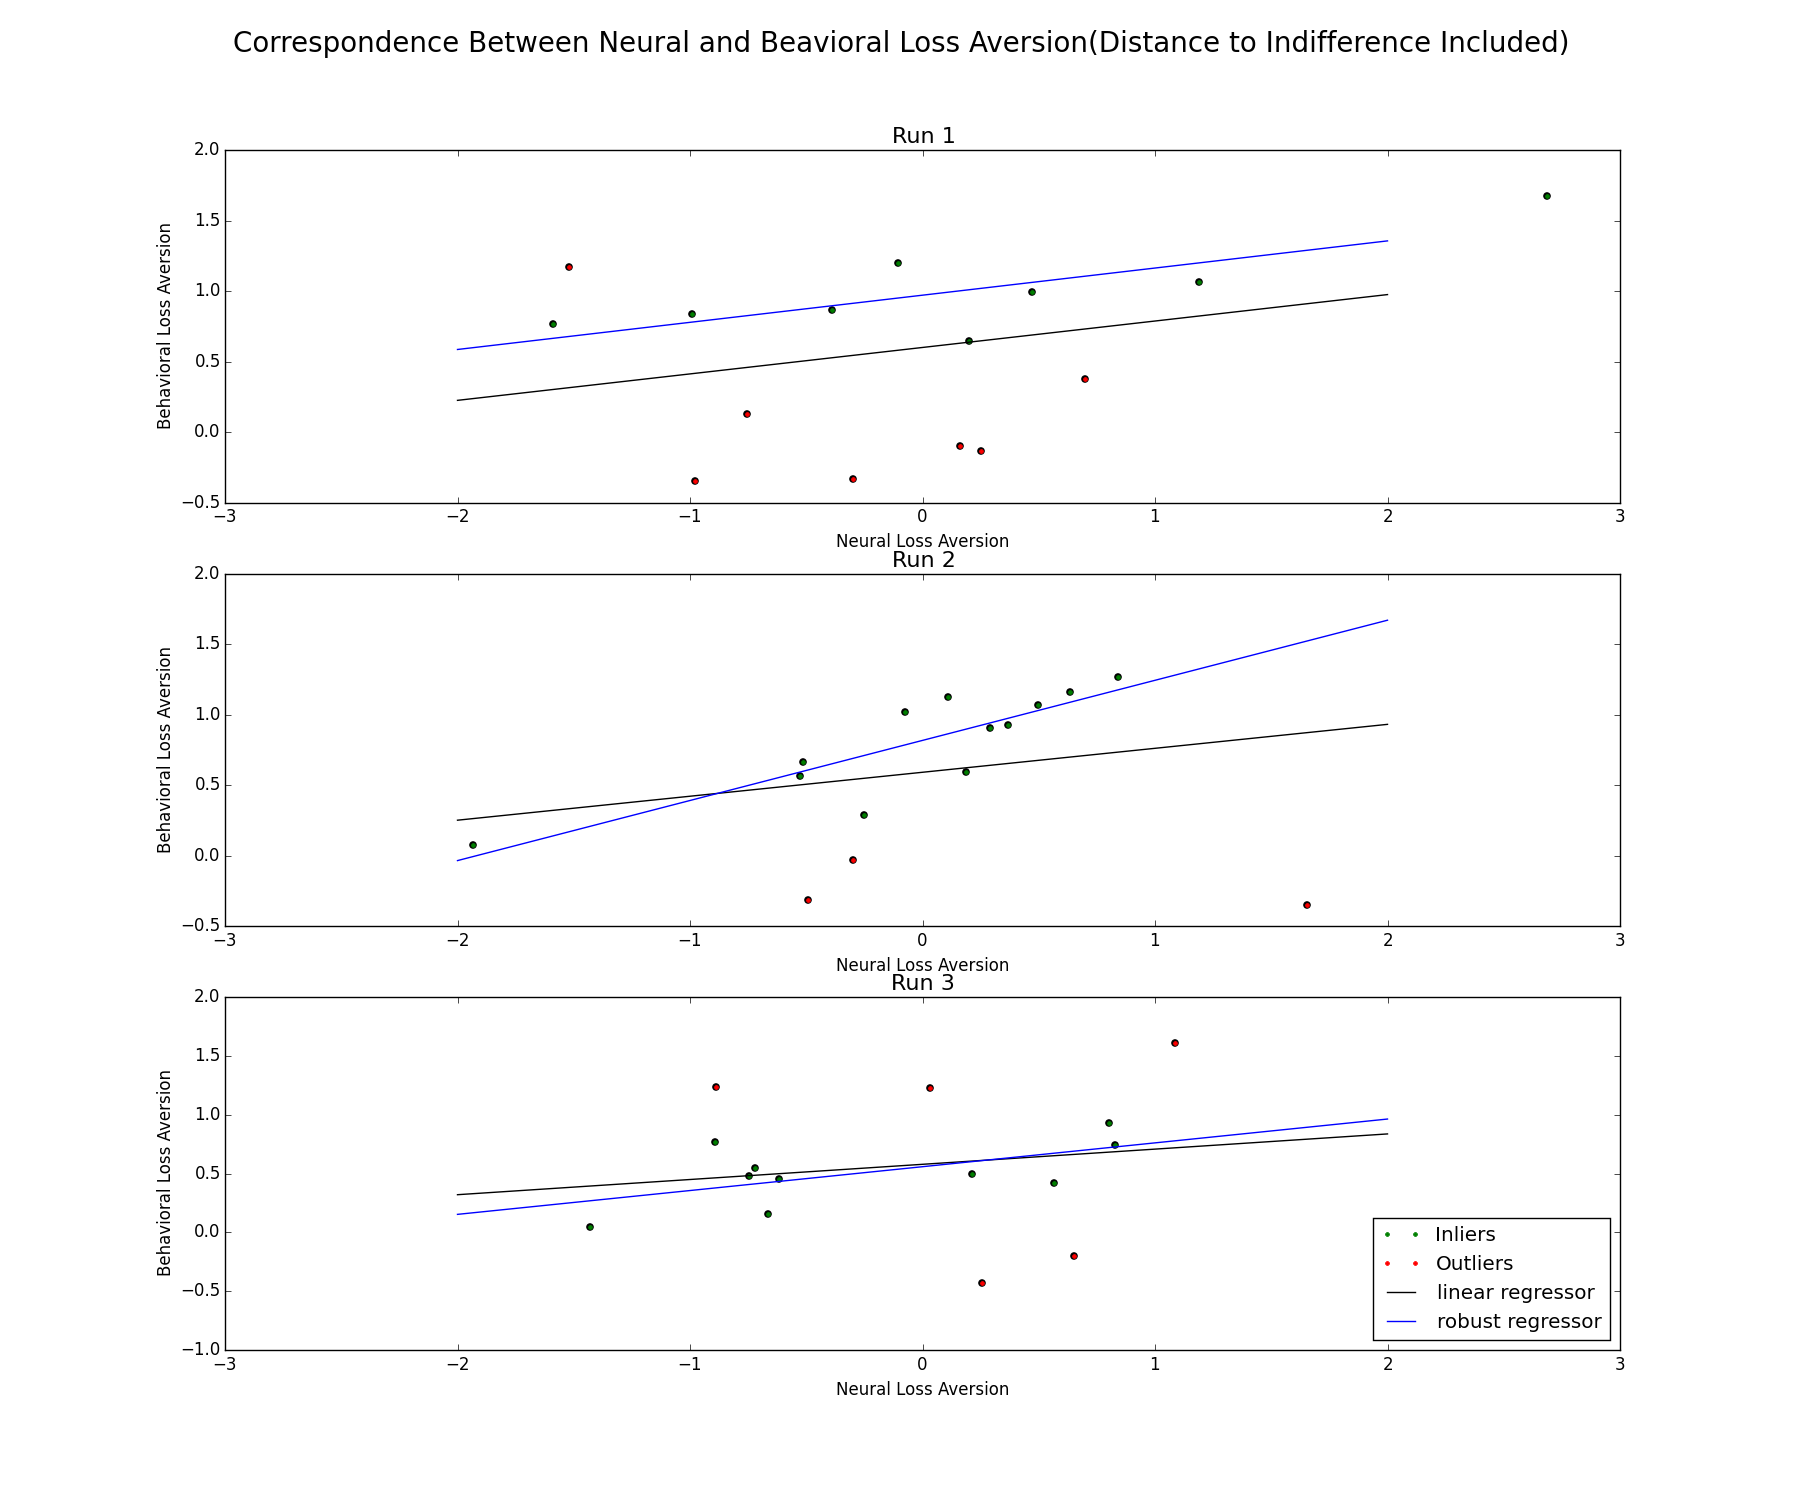
\includegraphics[width=100mm]{images/correlation_dist2indiff.png}               
\caption{Correspondence between neural and behavioral loss aversion (Include distance from indifference)}
\label{fig:cor1}
\end{figure}

\begin{figure}[h!]
\centering
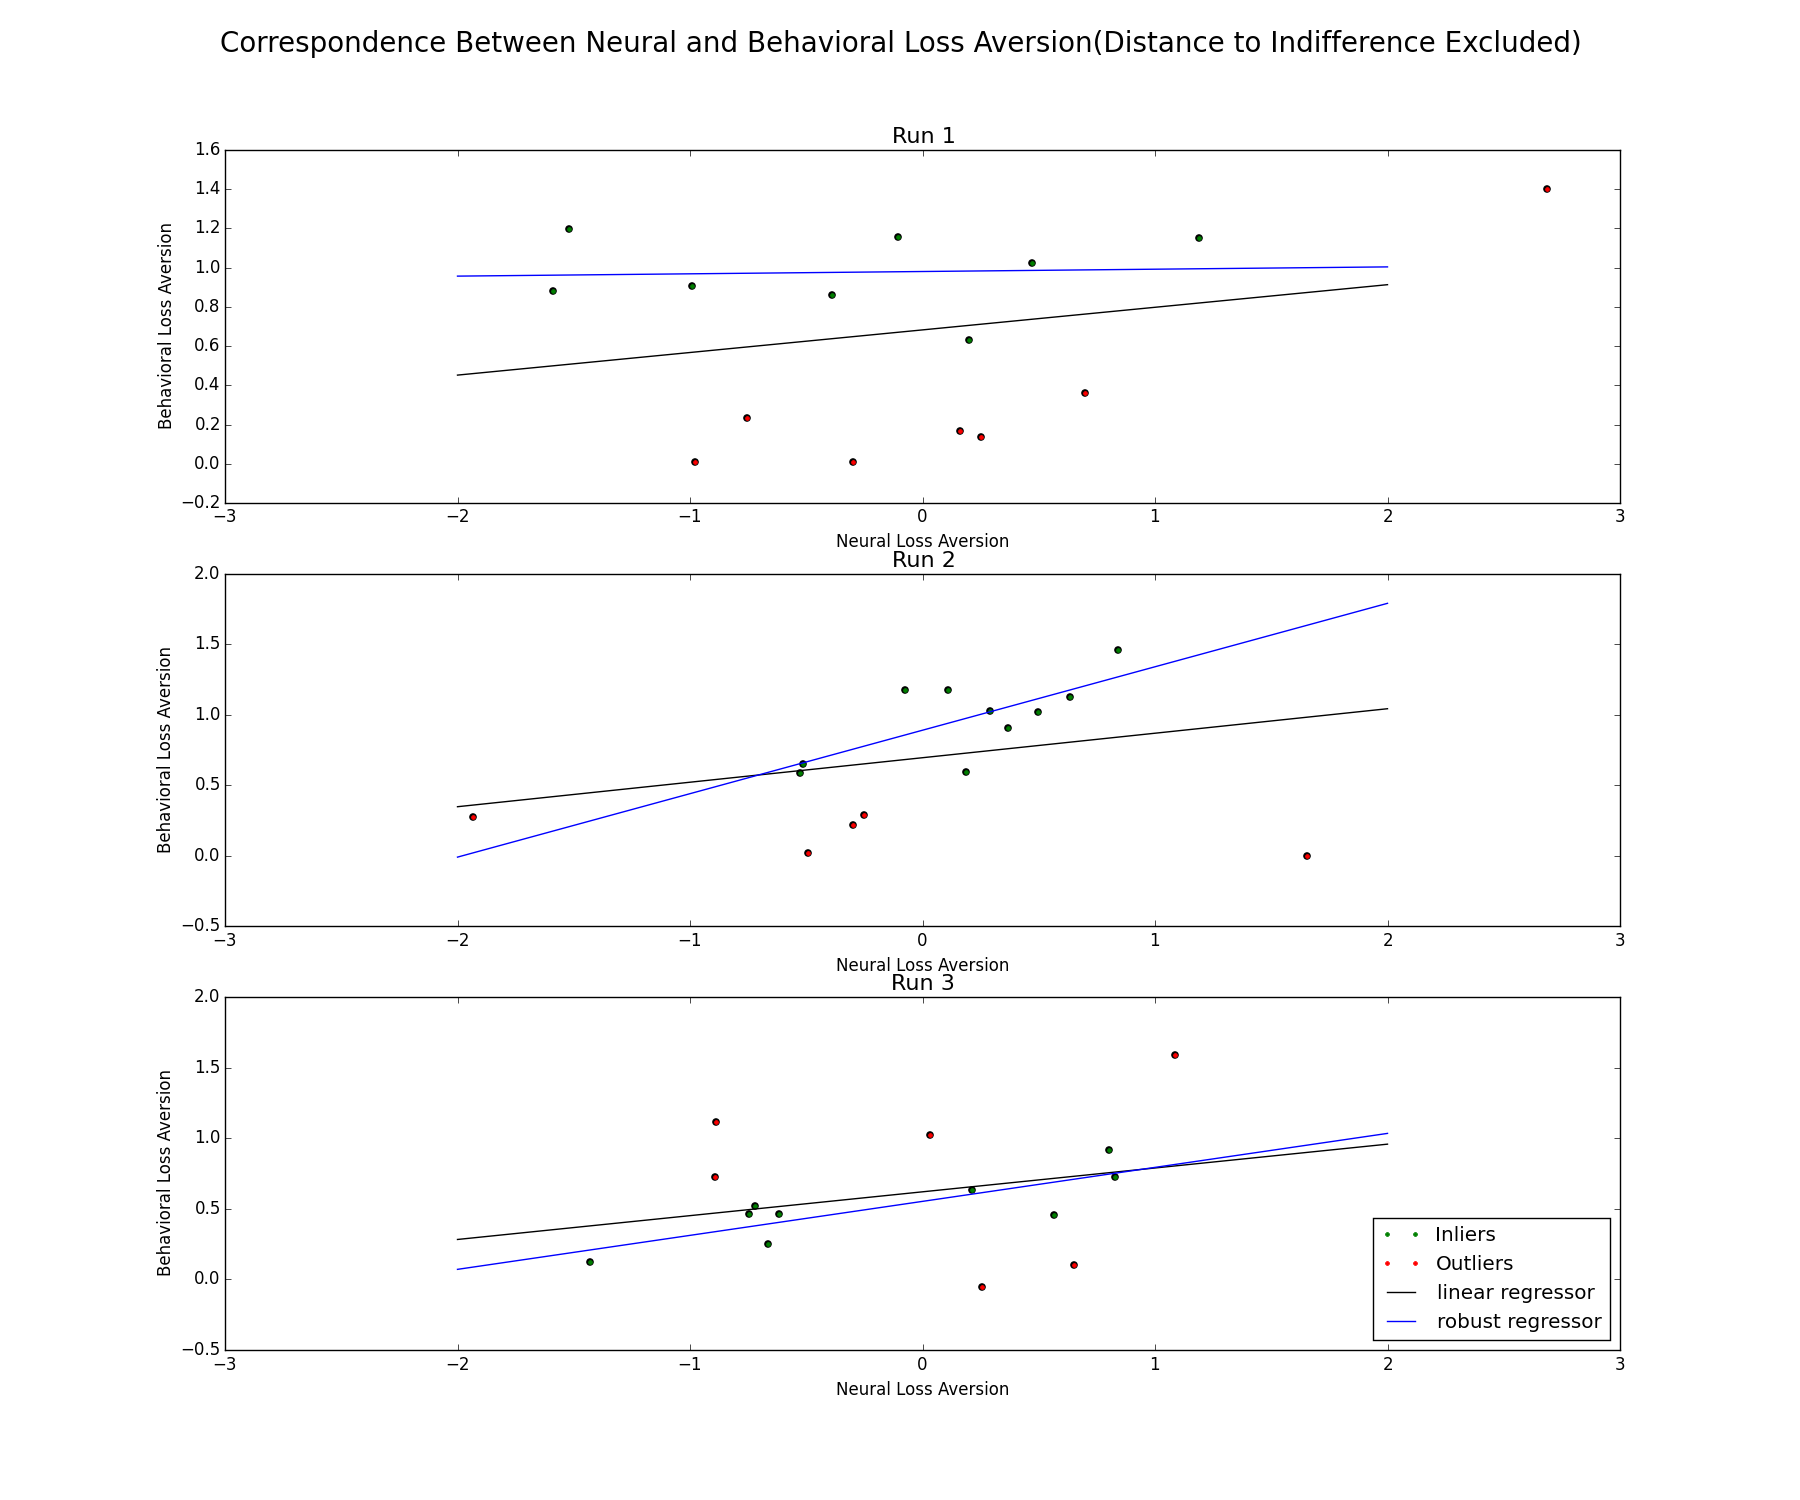
\includegraphics[width=100mm]{images/correlation_no_dist2indiff.png}               
\caption{Correspondence between neural and behavioral loss aversion (Exclude distance from indifference)}
\label{fig:cor2}
\end{figure}
